% Exact LaTeX recreation of the supplied Phase-1.pdf
% Compile with pdfLaTeX. Place member pictures in the same folder if required.

\documentclass[11pt,a4paper]{article}

\usepackage[a4paper,left=2.0cm,right=2.0cm,top=1.55cm,bottom=1.55cm]{geometry}
\usepackage[T1]{fontenc}
\usepackage{lmodern}
\usepackage{graphicx}
\usepackage{float}
\usepackage{xcolor}
\usepackage{array}
\usepackage{tabularx}
\usepackage{ragged2e}
\usepackage{enumitem}
\usepackage{fancyhdr}
\usepackage{tikz}
\usepackage{setspace}
\usepackage{url}

% -------------------------------------------------
% COLOURS
% -------------------------------------------------
\definecolor{TitleBlue}{RGB}{61,103,154}

% -------------------------------------------------
% GENERAL SETTINGS
% -------------------------------------------------
\setlength{\parindent}{0pt}
\setlength{\parskip}{0pt}
\renewcommand{\arraystretch}{1.0}

% The supplied document uses a clean sans-serif heading style
% and italic serif-style explanatory text.
\newcommand{\blueheading}[1]{%
    {\sffamily\color{TitleBlue}\fontsize{15}{18}\selectfont #1}%
}

\newcommand{\bluebigheading}[1]{%
    {\sffamily\bfseries\color{TitleBlue}\fontsize{16}{19}\selectfont #1}%
}

\newcommand{\instruction}[1]{%
    {\itshape\fontsize{10.5}{12.5}\selectfont #1}%
}

\newcommand{\answerbox}[2][3.0cm]{%
    \vspace{2pt}
    \noindent
    \fbox{%
        \begin{minipage}[t][#1][t]{\dimexpr\textwidth-2\fboxsep-2\fboxrule\relax}
            \vspace{1mm}
            \itshape #2
        \end{minipage}
    }
}

% -------------------------------------------------
% HEADER / FOOTER
% -------------------------------------------------
\pagestyle{fancy}
\fancyhf{}
\renewcommand{\headrulewidth}{0pt}
\renewcommand{\footrulewidth}{0pt}

\fancyhead[L]{%
    \sffamily\bfseries\itshape\fontsize{10.5}{12}\selectfont
    Data Structures and Programming in C++/DSCPP
}
\fancyhead[R]{%
    \sffamily\bfseries\fontsize{10.5}{12}\selectfont
    PROJECT PROPOSAL
}
\fancyfoot[R]{%
    \itshape\fontsize{10}{12}\selectfont
    Page \thepage
}
\setlength{\headheight}{14pt}
\setlength{\headsep}{23pt}
\setlength{\footskip}{24pt}

% -------------------------------------------------
% PAGE 1
% -------------------------------------------------
\begin{document}

\vspace*{4mm}

\bluebigheading{PROJECT AND TEAM INFORMATION}

\vspace{13mm}

\blueheading{Project Title}

\vspace{1mm}


\answerbox[1.0cm]{\bfseries\fontsize{12}{14}\selectfont
The Detective's Dossier}

\vspace{13mm}

\blueheading{Student / Team Information}

\vspace{2mm}

% Team information table
% Compact 4-member layout so all members remain on Page 1.
\noindent
\begin{tabularx}{\textwidth}{|>{\RaggedRight\arraybackslash}p{0.58\textwidth}|>{\RaggedRight\arraybackslash}X|}
\hline
\begin{minipage}[t]{\linewidth}
\vspace{1.5mm}
\textit{Team Name:}\\[-1mm]
\textit{Team ID:}
\vspace{1.5mm}
\end{minipage}
&
\begin{minipage}[t]{\linewidth}
\vspace{1.5mm}
\textit{Code Detektives}\\[-1mm]
\textit{DSCPP-III-2026-T027}
\vspace{1.5mm}
\end{minipage}
\\
\hline
\begin{minipage}[t][3.8cm][t]{\linewidth}
\vspace{1.5mm}
\textbf{Team member 1 (Team Lead)}\\[-1mm]
\textit{(Last Name, name: student ID: email, picture):}
\vspace{2.0cm}
\end{minipage}
&
\begin{minipage}[t][3.8cm][t]{\linewidth}
\vspace{1.5mm}
\textit{Bahuguna, Ashutosh -- 2510370440}\\
\url{ashutoshbahuguna2468@gmail.com}

\vspace{2mm}
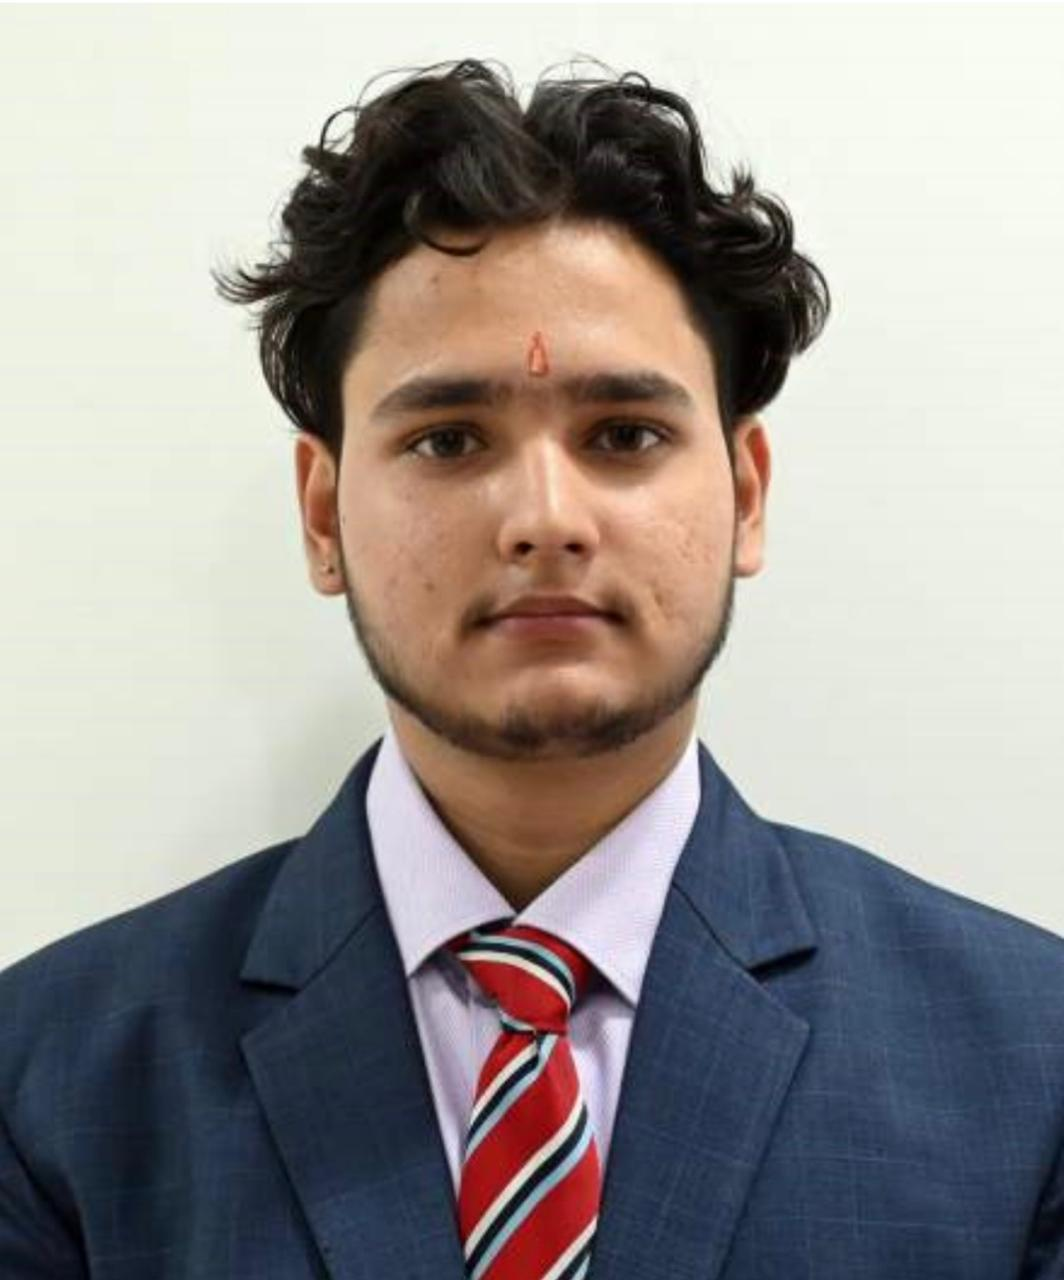
\includegraphics[width=3.0cm,height=1.5cm,keepaspectratio]{member1.jpeg}
\end{minipage}
\\
\hline
\begin{minipage}[t][3.8cm][t]{\linewidth}
\vspace{1.5mm}
\textbf{Team member 2}\\[-1mm]
\textit{(Last Name, name: student ID: email, picture):}
\vspace{2.0cm}
\end{minipage}
&
\begin{minipage}[t][3.8cm][t]{\linewidth}
\vspace{1.5mm}
\textit{Pundir, Snehal -- 2510370590}\\
\url{snehalpundir21052@gmail.com}

\vspace{2mm}
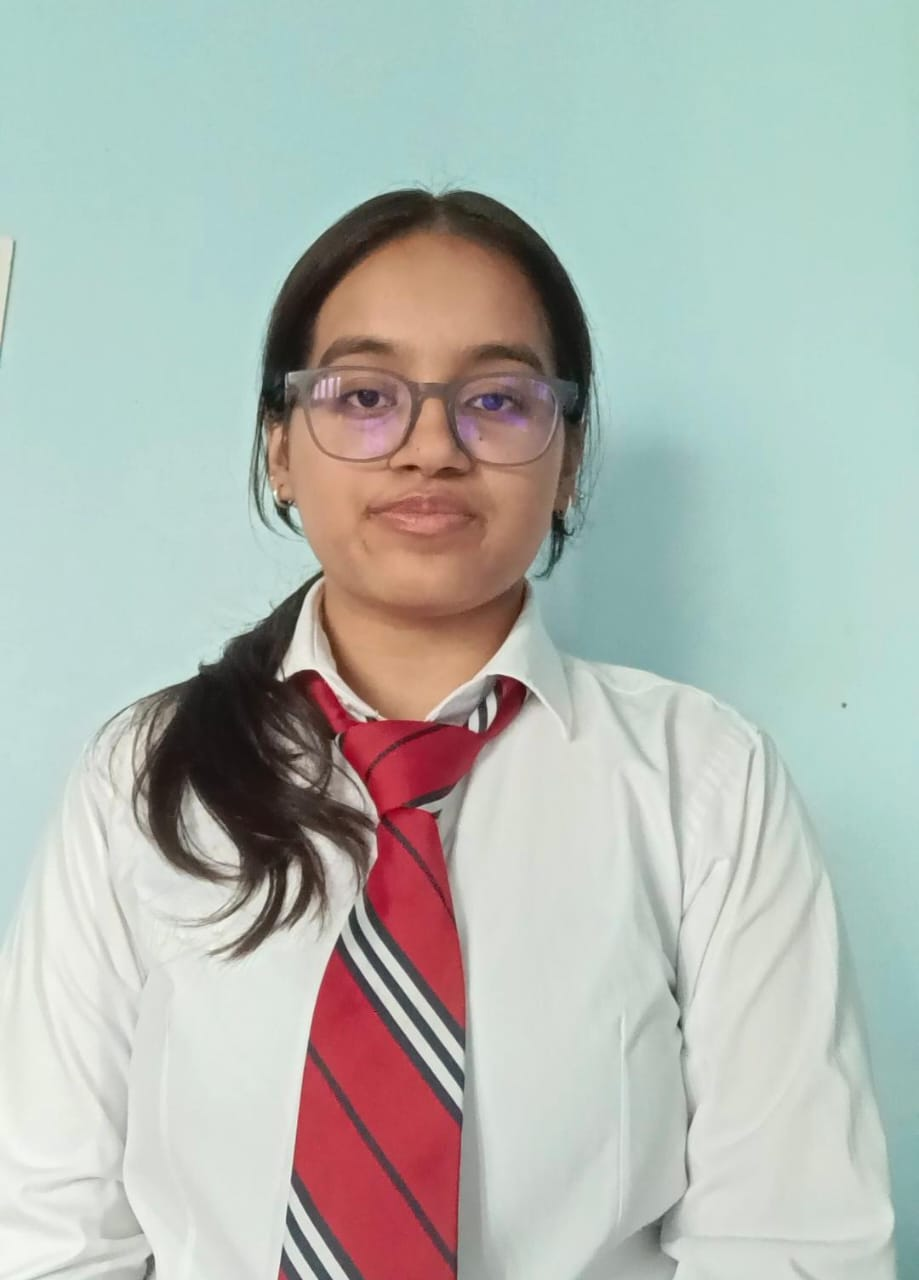
\includegraphics[width=3.0cm,height=1.5cm,keepaspectratio]{member2.jpeg}
\end{minipage}
\\
\hline
\begin{minipage}[t][3.8cm][t]{\linewidth}
\vspace{1.5mm}
\textbf{Team member 3}\\[-1mm]
\textit{(Last Name, name: student ID: email, picture):}
\vspace{2.0cm}
\end{minipage}
&
\begin{minipage}[t][3.8cm][t]{\linewidth}
\vspace{1.5mm}
\textit{Somraan, Vidhi -- 2510380302}\\
\url{Vidhisomraan@gmail.com}

\vspace{2mm}
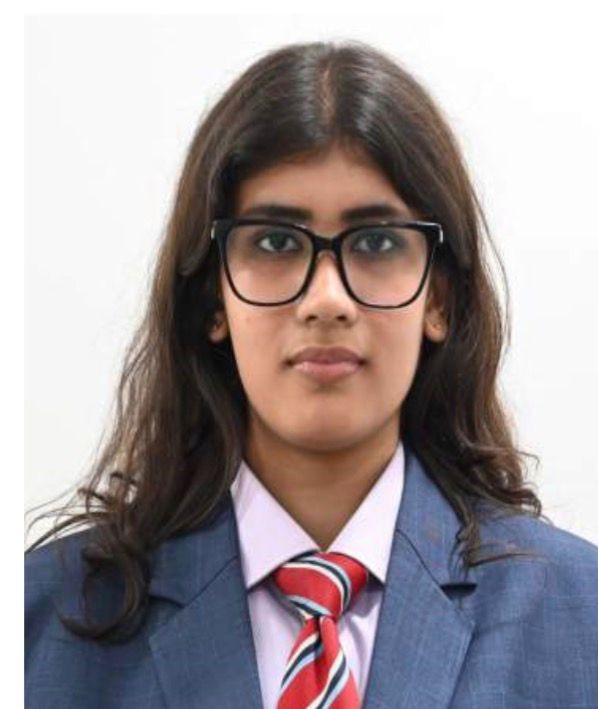
\includegraphics[width=3.0cm,height=1.5cm,keepaspectratio]{member3.jpeg}
\end{minipage}
\\
\hline

\end{tabularx}

\newpage

% -------------------------------------------------
% PAGE 2
% -------------------------------------------------

\bluebigheading{PROPOSAL DESCRIPTION (10 pts)}

\vspace{12mm}

\blueheading{Motivation (1 pt)}

\vspace{1mm}

\answerbox[4.1cm]{Murder mysteries and detective stories have always intrigued us because of the clues,suspects,observations and the intensity of it all.Growing up watching shows like CID and always having dreamt of solving a murder mystery added to our motive and hence we decided to create this project in the form of an interactive game.
In our project “The Detective’s Dossier”, players will take on the role of a detective in a 2D murder mystery game.They will have to collect clues,visit various locations,examine evidences and question the suspects.They will have to connect all the clues find the culprit.
Our primary reason to select this project was that it allows a practical use of Data Structures and Algorithms.Several DSA concepts can be used in the investigation.}

\vspace{12mm}

\blueheading{State of the Art / Current solution (1 pt)}

\vspace{1mm}


\answerbox[5cm]{Detective Murder Mystery games which are exiting often provide the players with the built-in cases which involves the clues, suspects,scenes and puzzles,this makes the players to find the culprits easily ,by just following the information .Thus, it fails to make the player feel like they are actually doing the detective work.

The Detective’s Dossier is designed as a more structured investigation game,where the person can actually actively explore the crime scenes and collect the clues and evidences.This game involves the practical implementation of the concepts of both Data Structures and Algorithms as well as Object Oriented Programming with C++.
Also ,the algorithms such as traversal algorithm,Dijkstra’s algorithm,hashing,stacks,queues and graph-based structures plays an important role as they can support navigation, represent locations and relationships and in efficient investigation management.}

\vspace{12mm}
\newpage
\blueheading{Project Goals and Milestones (2 pts)}

\vspace{1mm}

\answerbox[18cm]{
\textbf{Main Goals:}
\vspace{2mm}
\begin{itemize}[leftmargin=1.5em, itemsep=4pt, topsep=0pt]

\item To set up a 2D environment in which players can look into various murder cases.
\item To let players visit different locations and gather evidences.
\item To allow interactions between the player and the suspects through questioning.
\item To include Data Structures and Algorithms as an important part of our project’s logic.
\item To organise different game entities and modules through Object Oriented Programming.
\item To use SQLite to store all the data and player’s details.
\item To provide a result based on the player’s final choice.
\end{itemize}
\vspace{3mm}
\textbf{Milestones:}\\

\vspace{2mm}
\textbf{Phase I - Planning and Design}
\begin{itemize}[leftmargin=1.5em, itemsep=4pt, topsep=0pt]

\item Understand the problem and the requirements of the project.
\item Finalise the game’s concept and features.
\item Choose the technologies and various concepts that are to be used.
\item Draw the architecture of game and design the project.
\end{itemize}
\vspace{2mm}
\textbf{Phase II - Development}
\begin{itemize}[leftmargin=1.5em, itemsep=4pt, topsep=0pt]
\item Create a 2D interface using Qt.
\item Build the OOP structure of the game and the logic using DSA.
\item Set up SQLite database and work on the key aspects of investigation and gameplay.
\end{itemize}
\vspace{2mm}
\textbf{Phase III - Integration and Testing}
\begin{itemize}[leftmargin=1.5em, itemsep=4pt, topsep=0pt]
\item Make sure that all modules are connected.
\item Add some murder cases and test them.
\item Check DSA implementation and investigate the entire game.
\item Conduct user testing and make improvements to the final prototype.
\end{itemize}
}
\vspace{12mm}
\newpage
\blueheading{Project Approach (3 pts)}

\vspace{1mm}


\answerbox[14cm]{\vspace{2mm}
The system is build as a 2D interactive investigation game with the application of Object Oriented Programming with C++ ,Qt and SQlite.The project follows a modern approach in which it involves Graphical User Interface,Data Structures and Algorithms and application framework.
\vspace{2mm}
\textbf{• User Interaction}

The player will start the game by a login interface. After the successful login,the player will be able to the access the available investigation cases and continuing investigation process.

\vspace{2mm}

\textbf{• 2D Game Interface}

Qt will be used for the development of the investigation game. The interface will give the 
case selections ,  locations to explore,   evidence to inspect ,  find the suspects,   manage the clues.\vspace{2mm}

\textbf{• C++ and OOP}

The application will be implemented with the concepts of Object-Oriented Programming with C++ . use of appropriate encapsulation, inheritance and 
abstraction for the design \vspace{2mm}

\textbf{• DSA-Driven Investigation}

The major role for the making of the investigation game is the use of data structures and algorithms.the algorithms and techniques used are dfs,bfs and dijkstra’s algorithm ,  hashing, queue ,stack ,searching and sorting.\vspace{2mm}

Dijkstra's algorithm can be used for finding the shortest path between different locations.\vspace{2mm}

Hashing can be used to search suspects,evidences and other case details faster. Stacks can be used to keep track of the investigation history and to allow backtracking, while queue can be used for tasks which have to be dealt in a particular sequence.\vspace{2mm}

\textbf{• Database and Storage}

Sqlite is the local database being usd for the storage for the user account,  cases, clues and locations.\vspace{2mm}

\textbf{• Development and Testing}

The project will be carried out step by step by first creating and testing each module separately before integrating them.}


\newpage
% -------------------------------------------------
% PAGE 3
% -------------------------------------------------

\blueheading{System Architecture (High Level Diagram)(2 pts)}

\vspace{1mm}



\answerbox[14.5cm]{
\vspace{2mm}
 \begin{figure}[H]
    \centering
    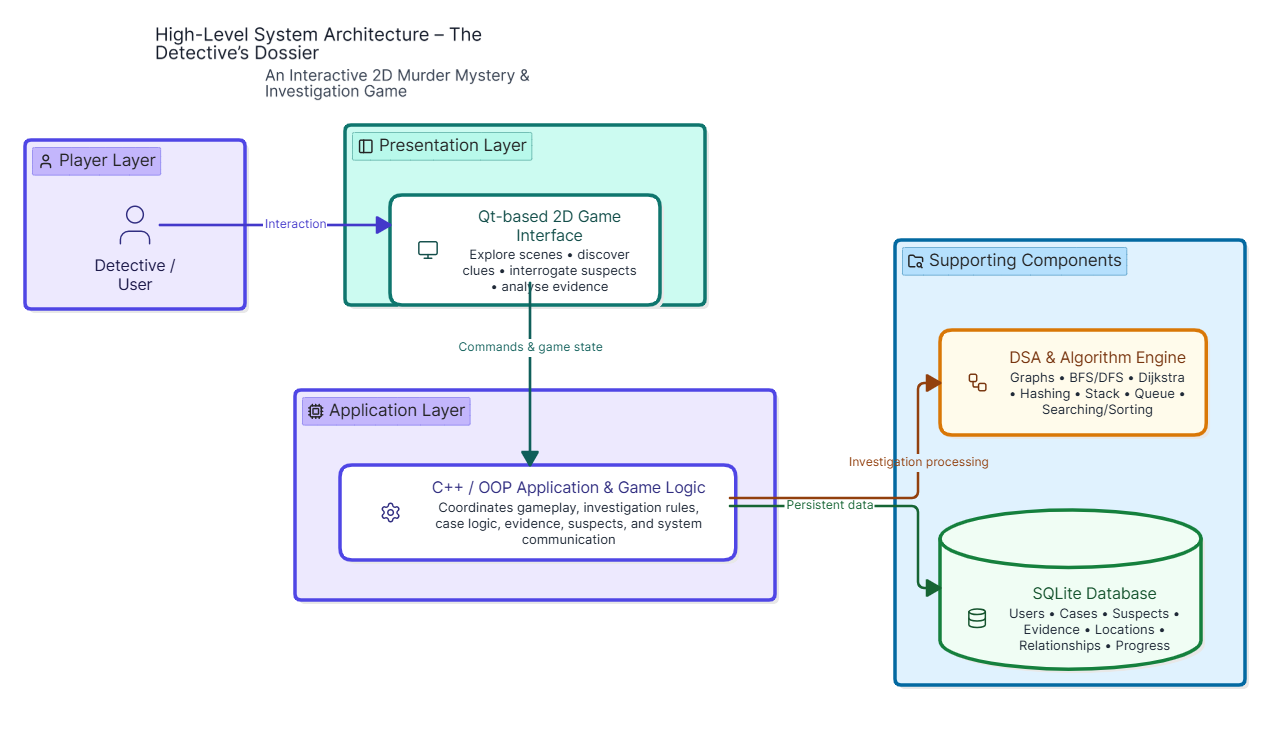
\includegraphics[
        width=\textwidth,
        height=25cm,
        keepaspectratio
    ]{architechture.png}
    \caption{High-Level System Architecture of The Detective's Dossier}
    \label{fig:architecture}
\end{figure}}
 \vspace{2mm}

\newpage
\blueheading{Project Outcome / Deliverables (1 pts)}

\vspace{1mm}

\answerbox[6.7cm]{

\vspace{2mm}

\textbf{Expected Deliverables}

\vspace{3mm}

\begin{itemize}[leftmargin=*, itemsep=2pt, topsep=2pt]

\item  A working 2D user interface using Qt.
\item A game structured using OOP concepts.
\item An investigation and navigation system based on DSA.
\item A number of murder mysteries that can be solved by the player.
\item Interaction between player,suspects,evidences and locations.
\item A system for final accusation and outcome of the case.
\item A working prototype that has been tested and integrated.

\end{itemize}}

\vspace{12mm}

\blueheading{Assumptions}

\vspace{6mm}


\answerbox[4cm]{\begin{itemize}[leftmargin=1.5em, itemsep=4pt, topsep=0pt]

    \item It will be a desktop based 2D interactive investigation game.
    \item It will run on sqlite and qt.
    \item The local database will store the clues, evidences and locations.
    \item It will select the dsa implementation according to the requirement of the gameplay and investigation .

\end{itemize}
}

\vspace{12mm}
\newpage
\blueheading{References}

\vspace{1mm}

\answerbox[5cm]{\begin{enumerate}[leftmargin=1.8em, itemsep=5pt, topsep=0pt]

    \item C++ Reference, cppreference:
    \texttt{https://en.cppreference.com/}

    \item Qt Documentation:
    \texttt{https://doc.qt.io/}

    \item SQLite Documentation:
    \texttt{https://www.sqlite.org/docs.html}

    \item T. H. Cormen, C. E. Leiserson, R. L. Rivest and C. Stein,
    \textit{Introduction to Algorithms}, MIT Press.

    \item R. Lafore,
    \textit{Object-Oriented Programming in C++}.

    \item Qt Creator Documentation:
    \texttt{https://doc.qt.io/qtcreator/}

\end{enumerate}}

\end{document}
